% proci.tex

\cleardoublepage
\chapter{LODESTAR}\label{chapter:LODESTAR}	
This chapter covers the optimal control program LODESTAR, which has been used to simulate the optimal trajectories of the rocket-scramjet-rocket system. The basics of optimal control and the optimal control methods used are presented, as well as the specific problem formulation used by LODESTAR.

The program LODESTAR (Launch Optimisation and Data Evaluation for Scramjet Trajectory Analysis Research) has been developed to aid with the simulation and trajectory optimisation of space launch systems.  LODESTAR optimises a trajectory towards a user-defined objective function, such as maximum payload-to-orbit, subject to constraints which bound the operational region of a vehicle. LODESTAR accurately models both rocket-powered and scramjet-powered vehicles in 6 degrees of freedom. LODESTAR contains multiple modules configured for the SPARTAN launch system, which are able to optimise trajectories for;

\begin{enumerate}
 \item The ascent of the first stage rocket.
 \item The ascent of the second stage scramjet-powered accelerator.
 \item The flyback of the second stage scramjet-powered accelerator.
 \item The ascent of the third stage rocket.
 \item Combined trajectories of multiple stages in any combination.
\end{enumerate}

LODESTAR performs optimisation using four classes of variables, states, controls, constraints and costs, which define the optimisation problem being solved. States are the variables which define the physical trajectory and are dependent on other states and the control variable. The control variables are independent in the solution space and can be modified freely by the solver algorithm within the prescribed limits.  Constraints bound the state and control variables to a well defined solution space and impose physical limitations on the vehicle such as structural or aerothermodynamic limits.
The constraints may also confine the state and control values to a specified value at a specific point in time, defining the flight conditions at the start and end points of a trajectory or phase. The cost function defines the target of the optimisation problem. This cost function may be any function which is defined by the states or controls of the optimisation problem. A solution to the optimisation problem is found when the cost is minimised to a suitable accuracy. 

LODESTAR is MATLAB based and utilises GPOPS-2, a proprietary pseudospectral method optimisation package.
GPOPS-2 requires that the vehicle model, constraints and cost function be modelled accurately as smooth, continuous functions. LODESTAR contains multiple modules that calculate the vehicle aerodynamic properties and run external simulations which then feed data back data to the pseudospectral solver for evaluation. Modules calculate the vehicle aerodynamic and engine output at each point along the trajectory. The vehicle model module takes this data and calculates the mass of the vehicle as well as the 6 degree of freedom motion derivatives of the vehicle along the trajectory. The cost is calculated using the state variables. The trajectory is evaluated to produce the final cost of the trajectory. The final step of each iteration is updating the state derivatives, which is performed by the dynamics file. The state derivatives and cost are evaluated by GPOPS-2 to determine if the trajectory has produced a suitable result. Figure \ref{fig:FlowChartSmall} illustrates an iteration of the pseudospectral solver.

 As this is an iterative process, the calculated system dynamics do not match the approximation exactly until convergence is achieved (This is a fundamental property of the pseudospectral method, see Section \ref{sec:PS}). Additionally, it is possible for GPOPS-2 to not be able to converge to an optimal solution. LODESTAR contains a number of verification modules which assess the optimised trajectory solution to ensure that the solution is indeed an optimal trajectory, and that the dynamics of the solution are accurate. 



\begin{figure}
	\centering
	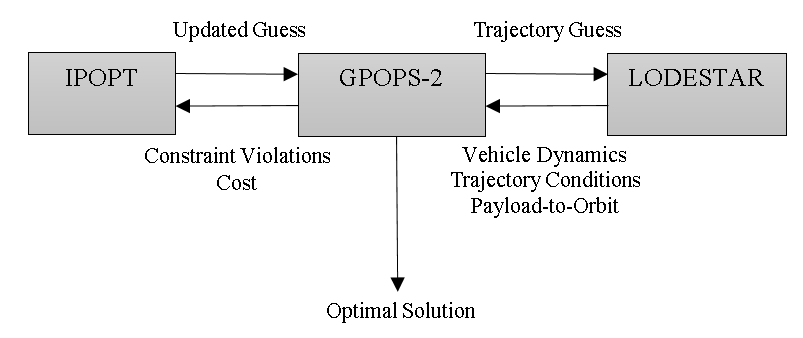
\includegraphics[width=0.5\linewidth]{figures/4_LODESTAR/FlowChartSmall}
	\caption{General work flow of the pseudospectral solver.}
	\label{fig:FlowChartSmall}
\end{figure}


\section{Optimal Control Problem Requirements}
The pseudospectral method and direct single shooting techniques used by LODESTAR are described in detail in sections \ref{sec:Optimisation}. Practically, the implementation of these techniques involves the specification of the dynamics of the system to be optimised, as well as the set of constraints and objectives which govern the optimisation problem. These constraints inform the optimiser of the bounds of the optimisation, and perform the functions of limiting the search space to the physically possible (eg. constraining altitude to be greater than ground level) as well as constraining the vehicle within its performance limits (eg. limiting the angle of attack). These constraints also come in the form of initial or terminal constraints, which define the initial conditions of the trajectory as well as any conditions which the trajectory must meet at termination. 

The pseudospectral method requires the specification of a set of 'state variables'. These state variables describe the physical dynamics of the system. In the pseudospectral method, the dynamics of the system are used as constraints on the optimal control problem;
\begin{equation} \label{eq:state2}
\dot{\textbf{x}}(\tau) = f[\textbf{x}(\tau),\textbf{u}(\tau)].
\end{equation}
Implementing the dynamics as constraints allows the optimiser to explore each state variable independently, greatly increasing the robustness of the optimal control problem. However, the constraints may be violated by the optimiser in the process of searching for an optimal solution. A violation of the physical dynamics constraints means that the dynamics of the system may not hold throughout the solution process, causing potential complications for the computational model of the vehicle. Much of the design of the vehicle simulation in this study is driven by the need for smooth, continuous interpolation schemes, and viable extrapolation regions ie. even if the solution is well within the range of all input data sets, the solver must be able to explore all regions within the set bounds. 

\subsection{GPOPS-2 Example - Brachistochrone Problem}
This section describes a short example optimal control problem solved in GPOPS-II. The purpose of this example is to demonstrate the effectiveness of the pseudospectral method and GPOPS-II, and to provide a simple example case to establish the terminology of an optimal control problem.  


The brachistochrone (from the Greek for 'shortest time') problem is a simple optimal control problem, which describes a ball rolling in two dimensions under gravity. The objective is to find the curve of descent which will minimise the time from point \textit{a}, where the ball is at rest, to point \textit{b}. It is assumed that gravity is constant and that there is no forces other than gravity acting on the ball. 

The analytical solution of this problem can be computed using the Euler-Lagrange equation as the equations describing a cycloid:

$x = A(\theta + \sin\theta) $,

$y=A(1 - \cos\theta)$

This problem has been solved as an example problem using GPOPS-2[cite Gpops XX]. Table XX describes the set-up of the optimal control problem in GPOPS-2. The dynamic equations for the Brachistochrone problem are:

$\dot{x} = v*cos(u)$,

$\dot{y} = v*sin(u)$,

$\dot{v} = g*sin(u)$.

\noindent These equations are provided to GPOPS-2 as the time-variant system model in this form. The control variable is set to be the descent angle. The initial constraints are defined to initiate the ball at rest at the origin, and the terminal constraints are defined to terminate the problem at coordinates of XX XX. The cost is set to minimum time, so that the solution will be the descent angle which minimises the time to get from the initial position, to the end position. 

\begin{table}
\centering
\begin{tabular}{|c|c|}
	\hline Primal Variables  & x Position\\& y Position\\& Velocity\\ 
	\hline Control Variables  & Angle of Descent\\ 
	\hline Initial Constraints  & Velocity\\ & x Position\\ & y Position\\
	\hline Terminal Constraints &  x Position\\ & y Position\\
	\hline Path Constraints & None \\ 
	\hline Target Cost & Minimum Time \\ 
	\hline 
\end{tabular} 
\end{table}


The GPOPS-2 solution to the Brachistochrone problem is shown in Figure \ref{fig:Brachistochrone}, matching the analytical solution almost exactly. This is expected in this case, as the dynamics of the basic Brachistochrone problem are very simple. As the dynamics become more complex, it is no longer possible to obtain an analytical solution. For more complex problems, more in-depth methods must be used to verify the optimal solution, outlined later in this chapter, in Section XX.  

\begin{figure}[ht]
\centering
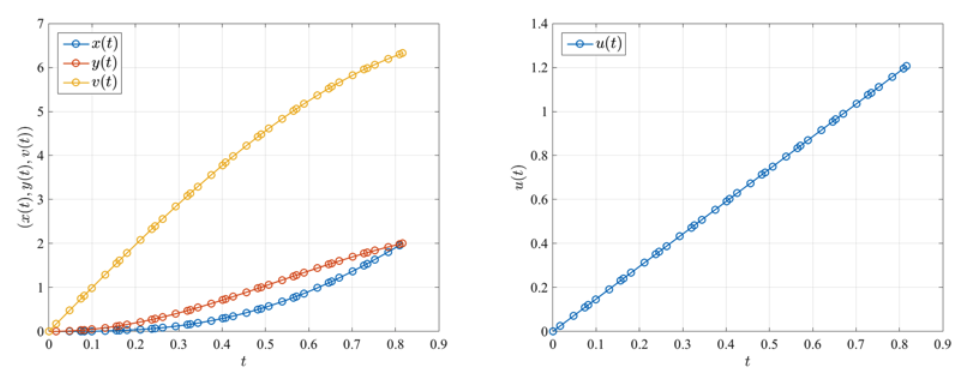
\includegraphics[width=0.9\linewidth]{figures/4_LODESTAR/Brachistochrone}
\caption{The solution to the brachistochrone problem, solved in GPOPS-2[CITATIONXX].}
\label{fig:Brachistochrone}
\end{figure}





\section{Rocket-Scramjet-Rocket Trajectory Optimisation}


The primary purpose of LODESTAR is to calculate a full trajectory optimisation of a rocket-scramjet-rocket launch vehicle for maximum payload-to-orbit. 




\begin{landscape}% Landscape page
	\begin{figure}[ht]
		\centering
		\includegraphics[width=0.9\linewidth]{"figures/4_LODESTAR/Ascent Flowchart"}
		\caption{The process of the rocket-scramjet-rocket trajectory optimisation.}
		\label{fig:AscentFlowchart}
	\end{figure} 
\end{landscape}


\subsection{Dynamic Model}


The dynamics of the vehicle are calculated in six degrees of freedom, with yaw constrained to zero. 
The dynamics of all stages are calculated using an geodetic rotational reference frame, written in terms of the angle of attack $\alpha$, bank angle $\eta$, radius from centre of Earth $r$, longitude $\xi$, latitude $\phi$, flight path angle $\gamma$, velocity $v$ and heading angle $\zeta$. The equations of motion are \cite{Josselyn2002a}:
\begin{figure}[ht]
\centering
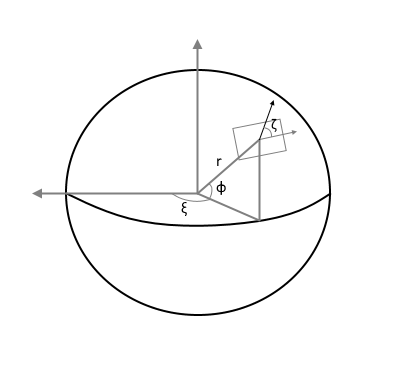
\includegraphics[width=0.7\linewidth]{figures/4_LODESTAR/global}
\caption{The Earth-fixed components of the geodetic rotational coordinate system.}
\label{fig:global}
\end{figure}
\begin{figure}[ht]
\centering
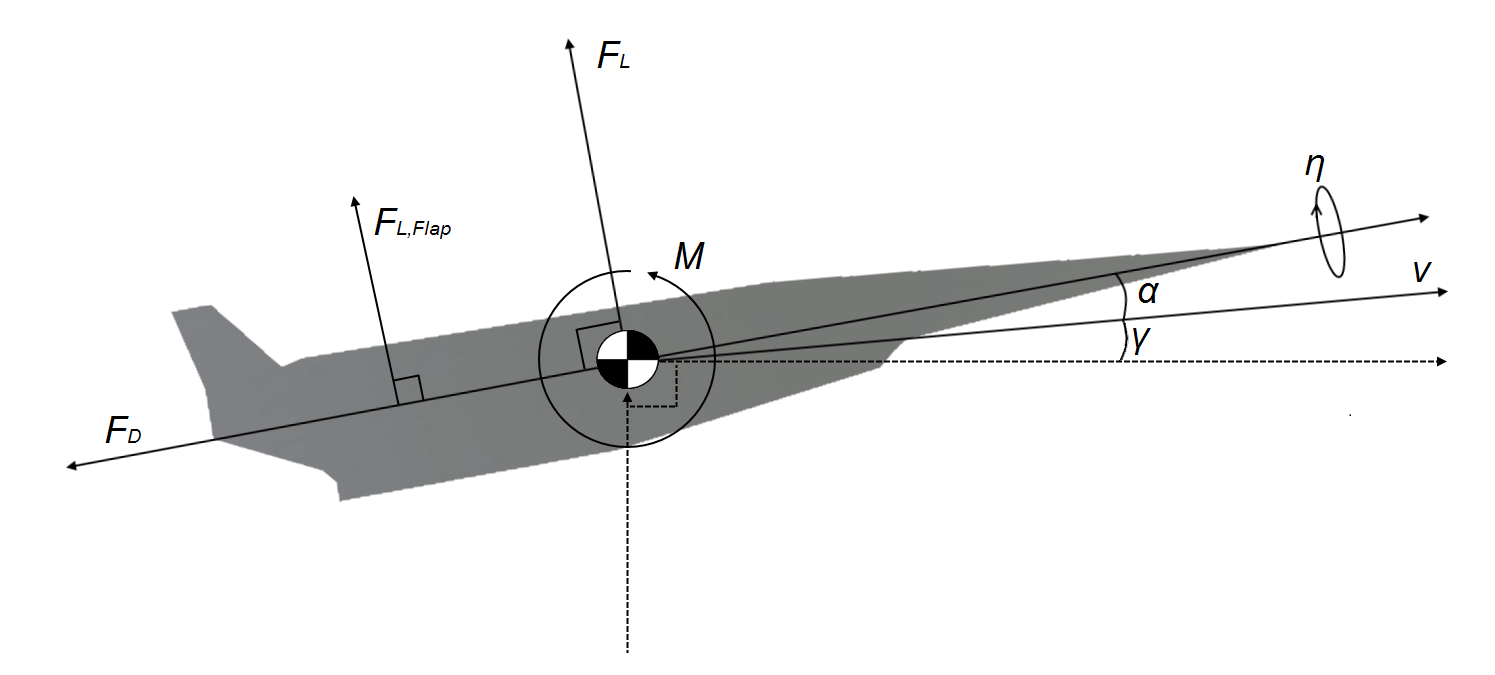
\includegraphics[width=0.9\linewidth]{figures/4_LODESTAR/Axes}
\caption{The vehicle-based components of the coordinate system.}
\label{fig:Axes}
\end{figure}


\begin{equation}
\dot{r} = v \sin \gamma
\end{equation}

\begin{equation}
\dot{\xi} = \frac{v\cos \gamma \cos \zeta}{r \cos \phi}
\end{equation}

\begin{equation}
\dot{\phi} = \frac{v\cos\gamma\sin\zeta}{r}
\end{equation}
\begin{equation}
\dot{\gamma} = \frac{T\sin\alpha \cos\eta}{mv} + (\frac{v}{r}-\frac{\mu_E}{r^2 v})\cos\gamma + \frac{L}{mv}
+ \cos\phi[2\omega_E \cos\zeta + \frac{\omega_E^2 r}{v}(\cos\phi\cos\gamma+\sin\phi\sin\gamma\sin\zeta)]
\end{equation}
\begin{equation}
\dot{v} = \frac{T\cos\alpha}{m}-\frac{\mu_E}{r^2}\sin\gamma - \frac{D}{m}
+ \omega_E^2 r\cos\phi(\cos\phi\sin\gamma-\sin\phi\cos\gamma\sin\zeta)
\end{equation}
\begin{equation}
\dot{\zeta} = \frac{T\sin\alpha \sin\eta}{mv \cos \gamma}-\frac{v}{r}\tan\phi\cos\gamma\cos\zeta +2\omega_E\cos\phi\tan\gamma\sin\zeta - \frac{\omega_E^2 r}{v\cos\gamma}\sin\phi\cos\phi\cos\zeta-2\omega_E\sin\phi 
\end{equation}

\subsection{Trajectory Connection Points}
The optimisation of a large, multi-vehicle problem therefore requires that the optimal control problem be broken down into multiple segments.
The aerodynamics, mass and propulsion mode of a launch vehicle may change significantly between stages. 
This creates discontinuities in the vehicle dynamics at the stage separation points. 
If these model variations are implemented directly into a single phase application of the pseudospectral method, they are likely to cause significant convergence issues, as the discontinuities in the system dynamics will be unable to be approximated by the underlying polynomial of the pseudospectral method. 

 The trajectory of the rocket-scramjet-rocket launch system has been broken down into the subsections shown in Figure \ref{fig:Traj}. 
 The trajectory of the rocket-scramjet-rocket vehicle is considered as four separate phases, within an overarching optimisation problem. In addition, there are three phases which are not directly controlled; the pre-pitch segment of the first stage, the unpowered section of the third stage ascent, and the final Hohmann transfer to orbit. These segments are not directly optimised, in order to increase computational efficiency and to improve the convergence of the optimal control solver. 
 Each segment is connected through a set of conditions, which ensure that the trajectory of the vehicle is continuous, and that the trajectory that is being flown is the one that is intended. 
The stage coupling conditions are described in Table \ref{tab:constraints}. 
The phases of the trajectory optimisation problem (segments \textcolor{red}{\rom{2}-\rom{5}}) are connected through the use of initial and end discontinuity constraints on each phase to be coupled, ie $\textbf{x}_{f1} = \textbf{x}_{02}, t_{f1} = t_{02}$. 
More specifics concerning the constraints on the initial and end states of each phase can be found in the following sections. 


\begin{figure}[ht]
	\centering
	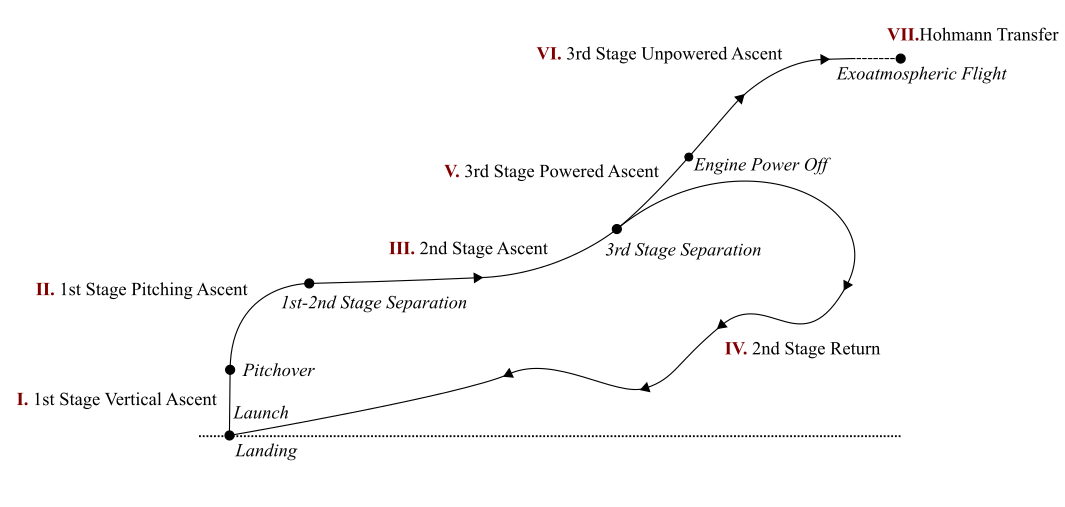
\includegraphics[width=1.\linewidth]{figures/4_LODESTAR/Traj}
	\caption{Illustration of the segmented launch profile.}
	\label{fig:Traj}
\end{figure}



\begin{table}[ht]


\begin{tabularx}{\linewidth}{|X|X|X|}
	\hline \textbf{Section} & Initial Conditions & End Conditions  \\ 
	\hline $1^{st}$ Stage Vertical Ascent (\textcolor{red}{\rom{1}}) & Must start at rest, at the predefined launch site. & Fly until pitchover conditions are met. \\ 
	\hline $1^{st}$ Stage Pitching Ascent (\textcolor{red}{\rom{2}}) & Start at pitchover conditions & - \\ 
	\hline $2^{nd}$ Stage Ascent (\textcolor{red}{\rom{3}}) & Must begin at first stage end conditions. & - \\ 
	\hline $2^{nd}$ Stage Return (\textcolor{red}{\rom{4}}) & Must begin at $2^{nd}$ stage ascent end conditions. & Must approach landing conditions at the initial launch site. \\ 
	\hline $3^{rd}$ Stage Powered Ascent (\textcolor{red}{\rom{5}}) & Must begin at $2^{nd}$ stage ascent end conditions.  & Must produce exoatmospheric flight at the termination of stage \rom{6}.  \\ 
	\hline $3^{rd}$ Stage Unpowered Ascent (\textcolor{red}{\rom{6}}) & Must begin at $3^{nd}$ stage powered ascent end conditions.  & Terminates when flight is parallel with Earth's surface.  \\ 
	\hline $3^{rd}$ Stage Hohmann Transfer (\textcolor{red}{\rom{7}}) & Must begin at $3^{rd}$ stage unpowered ascent end conditions. & Must attain prescribed orbit.  \\ 
	\hline 
	
\end{tabularx} 
\caption{Stage coupling conditions for combined trajectory optimisation.}
\label{tab:constraints}

\end{table}



\subsubsection{\textcolor{red}{\rom{1}.} First Stage Vertical Ascent}

LODESTAR optimises the ascent of the first stage rocket in two sections; pre and post-pitchover.
Initially, the first stage rocket is launched vertically, and continues vertically for a small amount of time, until pitchover is initiated. 
During the vertical launch the rocket is assumed to need no control, and is held at 0$^\circ$ angle of attack. 
The pitchover is defined to occur at 90m altitude and 30m/s velocity, rather than at a specific time.
This allows the pre-pitchover phase to be simulated separately, after the optimisation has been completed. 
If the initial mass is variable, the initial launch altitude will necessarily be slightly variable. This variation in launch altitude is small, on the order of ten meters or less. 

\subsubsection{\textcolor{red}{\rom{2}.} First Stage Pitching Ascent}


The post-pitchover trajectory is an angle of attack controlled phase in the optimisation routine, which is simulated from pitchover until second stage separation. During this phase, the launch system is allowed to fly at negative angles of attack, to assist in pitching. 
The fuel mass of the first stage rocket is unconstrained.
This approach is used on account of the selected first stage being able to reach the required range of altitudes and flight angles with only small fuel mass variations. 
Nevertheless, small variation in fuel mass can have an important effect on the capabilities of the first stage, influencing the velocity achievable at first to second stage separation, as well as the rate at which the rocket is able to pitch, and consequentially, the altitude and flight path angle range of the first stage.
A variable mass for the first stage launch vehicle is desired as the mass has large effects on the dynamics of the vehicle, effecting the trajectory angle change rate, as well as the acceleration and time of flight of the vehicle.
It is useful in the preliminary design stages to be able to optimise the mass of the first stage vehicle, allowing a less trial-and-error approach.
In the unconstrained mass case, the launch altitude is slightly variable, as LODESTAR starts optimisation from a set pitchover altitude and velocity, and the pre-pitchover trajectory is calculated to match the pitchover mass. 



\begin{table}[ht]
\centering
\begin{tabular}{|c|c|c|}
	\hline Optimisation Parameter  & Associated Variables & Allowable Values\\
	\hline Initial Constraints  & Velocity & 30m/s\\ & Altitude& 90m \\ & Latitude & $-12.16^\circ$ \\& Longitude & 136.75$^\circ$\\ & Trajectory Angle & 89.9$^\circ$\\ & Angle of Attack& 0$^\circ$\\
	\hline Terminal Constraints & $\textbf{x}_{f\textrm{\rom{2}}} - \textbf{x}_{0\textrm{\rom{3}}}$ & 0\\ & $t_{f\textrm{\rom{2}}} - t_{0\textrm{\rom{3}}}$ & 0\\
	\hline Path Constraints & Dynamic Pressure & 0kPa - 50kPa\\ 
		\hline Control Variables & $\ddot{\alpha}$ &\\ 
		\hline State Variables & Altitude & \\ & Velocity& \\  & Latitude& \\  & Longitude& \\  & Trajectory Angle& \\  & Heading angle& \\  & Total mass& \\  & Angle of Attack ($\alpha$)&  $-5^\circ$ - 5$^\circ$\\  & $\dot{\alpha}$& \\ 
	\hline 
\end{tabular} 

\caption{Optimisation setup of the first stage phase. \textcolor{red}{The other tables in this section will be modified to conform. I am currently unsure whether this table layout is clear.}}

\end{table}



\subsection{\textcolor{red}{\rom{3}.} Second Stage Ascent Trajectory}




LODESTAR is able to optimise the trajectory of airbreathing accelerators in the supersonic or hypersonic regime. LODESTAR is able to optimise for a range of optimisation metrics, including a maximum payload-to-orbit and constant dynamic pressure.  
The trajectory of the SPARTAN scramjet-powered accelerator has been simulated in LODESTAR. 

\begin{table}[ht]
\begin{tabular}{|c|c|}
	\hline Initial Constraints  & Velocity \\ & Fuel Mass  \\ & Latitude \\ & Longitude \\ 
	\hline Terminal Constraints & Fuel mass \\ & Heading Angle \\ 
	\hline Path Constraints & Dynamic Pressure \\ 
	\hline Target Cost & Maximum Payload-to-Orbit \\ 
			\hline Control Variables &  \\ 
			\hline State Variables &  \\ 
	\hline 
\end{tabular} 

\end{table}

\subsection{\textcolor{red}{\rom{4}.} Second Stage Return Trajectory}
After releasing the third stage rocket, the scramjet-powered second stage must return back to an area close to the initial launch site.
During the fly-back, the SPARTAN cannot exceed its dynamic pressure limit of 50kPa. 
The SPARTAN must land on the ground with minimum velocity, within close proximity to the launch area. It is assumed that a landing strip is available at the spot where the SPARTAN lands. The SPARTAN is required to land within a set radius of the launch site. This constraint is;
\begin{equation}
(\phi_{end} - \phi_{launch})^2 + (\xi_{end} - \xi_{launch})^2 - r^2 \leq 0
\end{equation}

\textcolor{red}{detail throttling}


\begin{tabular}{|c|c|}
	\hline Initial Constraints  & Altitude \\ & Velocity\\ & Flight Path Angle\\ & Heading Angle\\ & Latitude\\ & Longitude\\ 
	\hline Terminal Constraints &  Distance From Launch Site \\ 
	\hline Path Constraints & Dynamic Pressure \\ 
	\hline Target Cost & Minimum End Velocity \\ 
				\hline Control Variables &  \\ 
				\hline State Variables &  \\ 
	\hline 
\end{tabular} 




\subsection{\textcolor{red}{\rom{5}.} Third Stage Powered Ascent}

The trajectory of the third stage rocket is only directly optimised during the powered section of its trajectory. During powered flight, the engine is used to control the third stage vehicle. After this point, the engine is cut, and the third stage is assumed to not have sufficient aerodynamic control to manoeuvre. 

The third stage rocket is constrained to an angle of attack of less than 20$^\circ$. This is assumed to be the maximum controllable angle of attack possible for the third stage rocket.   
Additionally, a maximum normal force restriction is placed on the third stage. Previous studies flew the third stage rocket at a constant 10$^\circ$ angle of attack, and initially released the rocket at 50kPa. 
For this study, it is assumed that 10$^\circ$ angle of attack produces the maximum allowable normal force at 50kPa, to prevent the rocket from being released into an environment which could exceed its structural limitations. The maximum allowable normal force is calculated at the release Mach number, and set as a path constraint. 
The heat shield is released once the rocket reached a dynamic pressure of 10Pa, where it is assumed that atmospheric effects will have ceased to have a major thermal effect. 

\begin{tabular}{|c|c|}
	\hline Initial Constraints  & \\ 
	\hline Terminal Constraints & None \\ 
	\hline Path Constraints & Angle of Attack \\ 
	\hline Target Cost &  \\ 
				\hline Control Variables &  \\ 
				\hline State Variables &  \\ 
	\hline 
\end{tabular} 


\subsection{\textcolor{red}{\rom{6}.} Third Stage Unpowered Ascent}

The unpowered section of the trajectory is simulated from the end of the controlled section of the trajectory, using a second order Taylor series approximation. This integration ceases when the flight path angle reaches 0$^{\circ}$. After this point, a circularisation burn is performed. The third stage is required to deliver the payload into heliosynchronous orbit. The third stage must achieve an inclination of of 97.63$^\circ$.



\subsection{\textcolor{red}{\rom{7}.} Hohmann Transfer}

After the circularisation burn, the rocket will still be in a very low orbit. In order to reach a heliosynchronous orbit of 567km, the orbit of the third stage rocket must be raised. 
To this end, the final manoeuvre performed by the third stage rocket is a Hohmann transfer. A Hohmann transfer is the most fuel efficient way to raise a spacecraft from one circular orbit to another. 

Following circularisation, the third stag engine is reignited (or remains ignited) and the third stage manoeuvres into an appropriate elliptical orbit. 



The payload-to-orbit is determined by calculating the mass of the vehicle at the end of the Hohmann transfer. The structural mass is removed, and the remaining mass is taken to be the payload-to-orbit capability of the vehicle.

\textit{The Hohmann transfer will be detailed here. Standard Hohmann transfer.}



\section{Optimality Conditions}

LODESTAR provides the capacity to validate the optimal solution provided by the pseudospectral method solver. This partial validation is used to determine whether the pseudospectral method solver has converged close to an optimal solution of the nonlinear programming problem. It is particularly useful to validate that the optimality and constraint tolerances which have been chosen are sufficiently small, or to check whether the pseudospectral method solver has approached an optimal solution in the case that the defined tolerances are not able to be reached.   
This partial validation is achieved through the examination of four key metrics; the IPOPT constraint violation and dual infeasibility parameters; the Hamiltonian necessary condition for optimality; the state derivatives; and finally a forward simulation. 

The first metric to be checked is the IPOPT constraint violation and dual infeasibility parameters[CITEXX intro to Ipopt]. The constraint violation parameter is a measure of the infinity-norm ($L_\infty-norm$) of the constraints of the problem. This factor has to be suitably small in order to indicate that the constraints of the problem to have been met. While the permissible magnitude of this factor changes with each individual problem, it is always desirable for this factor to be as small as possible. For this study only solutions with $L_\infty-norm(inf-pr) < 10^{-4} $ are accepted as having satisfied the imposed constraints. The dual infeasibility is a Karush-Kuhn-Tucker condition[CITEXX], which is a necessary condition for optimality. A dual feasible solution indicates that the dual problem is at least a lower bound on the optimal solution, $p^\star$, ie. $p^\star \geq g(\lambda,v)$. For more details on duality see [Find good citationXX].
A low dual infeasibility indicates that the solution has approached an optimal solution. Again, the magnitude of this value is variable with each problem, though as a problem becomes more complex, the ability to converge towards an optimal solution diminishes. For the problem in this study, $L_\infty-norm(inf-du) < 0 $ are accepted due to the highly complex nature of the vehicle model. In this study it is accepted that a given solution may not approach the global optimum, and multiple solutions are calculated to mitigate the error caused by the problem complexity, with the 'most optimal' solution selected. 

citation for optimality conditions, well explained https://ieeexplore.ieee.org/stamp/stamp.jsp?arnumber=1655436

The Hamiltonian of the optimal control problem is defined as 
\begin{equation}
H(x(t),u(t),\lambda(t),t) = \lambda^T(t)f(x(t),u(t)) + L(x(t),u(t))
\end{equation}
The Hamiltonian of the optimal control problem is investigated as a partial verification that the first order necessary conditions hold. Due to the unconstrained end time of the trajectory problems, $H\equiv 0 $ \cite{Pucci2007}. The Hamiltonian is defined as: $H(x(t),u(t),\lambda(t),t) = \lambda^T(t)f(x(t),u(t))+L(x(t),u(t))$.
This is calculated using LODESTAR and the Hamiltonian condition is able to be verified. The Hamiltonian will likely not be exactly equal to zero along the trajectory. This is due to the heuristic nature of the solver, which will approach close to an optimal solution, but never reach it exactly. A sufficiently small Hamiltonian indicates that the end solution approaches an optimal solution, and may be a candidate as an optimised trajectory case. 


The pseudospectral method considers the dynamics of the system as constraints on the optimal control problem, and solves across the entire trajectory simultaneously. This causes the physical system dynamics to have an associated margin of error, ie. $\dot{x} = f(x)$ will only hold to a certain degree of accuracy. For a well converged solution, this margin of error will be negligibly small, and the dynamics of the system will be consistent with realistic Newtonian dynamics. However, when the problem is not well converged, the dynamics of the system may have a large error.
A check is performed on each state to affirm that the derivative of the approximated state is equal to the derivative supplied by the vehicle model. This checks that the solver has converged to a solution which satisfies the vehicle dynamics at each individual node. 
The state feasibility of the solution is checked through a comparison of the state derivatives, $\dot{x} = f(x,u)$. $\dot{x}$ is first determined through numerical differentiation of the state variables over the solution time. Then $f(x,u)$ is determined using the dynamics of the system and vehicle model, in the same way that $f(x,u)$ is input to the pseudospectral solver. Examination of the error between the 'expected' state derivatives, and the numerical approximation of the derivatives, $\dot{x} - f(x,u)$, allows the accuracy of the system dynamics to be verified. 



 However, to be certain that the system is behaving as it should be, a full forward simulation is necessary. This forward simulation starts at the initial conditions prescribed by the pseudospectral method solver, and propagates the dynamics of the system forward in time using numerical approximation. The forward simulation uses only inputs of the control sequence, as solved for by the pseudospectral method. 
This checks that the flight path will follow the optimised path using the calculated control inputs. This is the most complete test of the optimal solution. However, in some cases calculating a forward solution may be problematic. The pseudospectral method has a limited number of nodes, potentially spread across relatively large time steps. Due to the high accuracy of the polynomial approximation, the pseudospectral method is able to maintain accuracy over large time steps. However, a forward simulation may \textcolor{red}{not lose accuracy reprase}lose accuracy when applied to the optimal solution, causing minor deviations, particularly when the states or controls are changing rapidly. These minor deviations may propagate themselves forward, causing significant deviation in the forward simulation. This can in some cases also cause the forward simulation to appear close to the optimial solution, when it should deviate. For this reason, a forward simulation is a good final check of an optimal solution, but knowledge of the system dynamics must be used, along with the other verification methods, to ascertain if a solution has converged sufficiently. 

\textcolor{red}{It may be useful to include example images here}

